\achapter{3}{Applications}\label{sec:metric_applications}


\vspace*{-17 pt}
\framebox{\hspace*{3 pt}
\parbox{4.7 in}{\begin{fqs}
\item 

\end{fqs}} \hspace*{3 pt}}

\vspace*{13 pt}

\csection{Introduction}       % Enter section title between curly braces

Although topology can be an abstract topic, it has many applications. Indeed, an Internet search on the topic of applications of topology turns up may examples. In this section we will discuss a few of these many examples in detail.

\csection{The Hamming Meteric}

 In our society, a great deal of information is communicated electronically. Bank transactions, television programs, military communications, cell phone calls, digital images, and almost any interchange one can think of either can be or is digitized and transmitted electronically. In many situations we need to compare one set of data to another (e.g., Internet searches for text strings or image matches, DNA strands), and metrics are often used for this purpose. 
 
Let us begin by discussing how information can be digitized. Computers work in a binary system, that is they recognize only zeros and ones. So to digitize a text message, the message must be converted into a string of zeros and ones. We can convert an alphabet into numbers by assigning a number to each letter, say A is assigned 1, B is assigned 2, and so on. We can also assign numbers to spaces and other characters. These numbers are then converted into binary. What results is that digitized messages are elements of the set $X^n$ for some positive integer $n$, where $X = \{0,1\}$. Often, instead of writing an element in $X^n$ as an ordered $n$-tuple, we just string the entries of an $n$-tuple together. So a short message (an element of $X^{27}$) might look like 
\[100010100100111010100111010.\]
We will call any string of zeros and ones like this a \emph{word}. Just like in the English language, where not every combination of letters corresponds to words that make sense, not every word is recognizable as part of an intelligible message. The collection of all intelligible words is called a \emph{code}. So a code is just some subset of $X^n$ that parties agree are sensible words. The words in a code are called \emph{code words}. 

When transmitting information through electronic media from one party to another there are three basic problems to be considered. If the information is important, the sending party must decide how to scramble, or \emph{encode}, the information to make it secure. A related problem is to ensure that the receiving party can unscramble, or \emph{decode}, the message. We won't address these two issues here, but rather focus on the third. Whether or not a message is encoded, there is always the possibility that the message may somehow be garbled during transmission. This can happen in several ways: operator error, noise can be introduced in a message, information can be lost during transmission, and data can be altered during transmission. Consequently, we need to be able to detect when an error has occurred, and we need to be able to correct any detected errors. We won't get into error detection, but will assume that if a message that has been received does not make sense, then an error has occurred. The problem, then, is how to correct the error. When an error has occurred, we will have received a word or words that are not code words. If we assume that the number of errors is small, then it makes sense to correct a received message by replacing any non-code words with the code words that are closest to them. To do this, we need a way to measure distance between words. One way is to use the Hamming metric. 

We will denote a word (a string of zeros and ones) in the form $(x_1, x_1, \ldots, x_n)$. If two words have a different number of characters (the value of $n$), we can pad the shorter word on the left with a string of zeros to make them have the same number of characters. So we can then consider all of our words as elements of $X^n$ for some fixed value of $n$. 



\begin{definition} Let $x = (x_1, x_2, \ldots, x_n)$ and $y = (y_1, y_2, \ldots, y_n)$ be words in $X^n$. The \textbf{Hamming distance} $d_H$ between $x$ and $y$ is 
\[d_H(x,y) = \sum_{i=1}^n \la x_i-y_i \ra.\]
\end{definition}



Recall that for each $i$ both $x_i$ and $y_i$ are either 0 or 1. So 
\[\la x_i-y_i \ra = \begin{cases} 0 &\text{if } x_i=y_i \\ 1 &\text{ if } x_i \neq y_i. \end{cases}\]
In other words, $d_H(x,y)$ counts the number of components at which $x$ and $y$ are different. Note also the $d_H$ is just the taxicab metric on $X^n$ and so is a metric. 



\begin{activity} Let 
\begin{center}
\begin{tabular}{llll}
$c_1 = (0,0,0,0,0,0)$, 	&$c_2=(0,0,0,0,1,1)$, 	&$c_3=(0,0,0,1,0,1)$, 	&$c_4=(0,0,1,0,0,1)$, \\
$c_5=(0,0,0,1,1,0)$, 		&$c_6=(0,0,1,0,1,0)$, 	&$c_7=(0,0,1,1,0,0)$, 	&$c_8=(0,0,1,1,1,1)$
\end{tabular}
\end{center}
and let 
\[C = \{c_1,c_2,c_3,c_4,c_5,c_6,c_7,c_8\}\]
be a code in $X^6$. 
\ba
\item Find $d_H(c_2, c_8)$.

\item Suppose we receive the message 
\begin{equation} \label{eq:message}
(0,0,0,1,1,1) \ (0,0,0,1,0,0) \ (0,0,1,1,1,0) \ (0,0,0,0,1,1) \ (0,0,1,0,0,1).
\end{equation} 
	\begin{enumerate}[i.]
	\item How do we know that an error has occurred in transmission?

\begin{comment}
Note that $(0,0,0,1,1,1)$, $(0,0,0,1,0,0)$, and $(0,0,1,1,1,0)$ are not in $C$. Since $C$ contains all of the possible words in our message, we know that there are errors in our message. 

\end{comment}

	\item To correct the errors in this message, we replace the incorrect words with the code word(s) in $C$ closest to them. Correct this message. (Note that there may be more than one possible substitution. Find all of the possibilities.)
	


	\end{enumerate}

\ea

\end{activity}

\begin{comment}

\ActivitySolution

\ba

\item Since $c_2$ and $c_8$ differ only in the third and fourth components, we have that $d_H(c_2,c_8) = 2$. 

\item Suppose we receive the message 
\begin{equation} \label{eq:message}
(0,0,0,1,1,1) \ (0,0,0,1,0,0) \ (0,0,1,1,1,0) \ (0,0,0,0,1,1) \ (0,0,1,0,0,1).
\end{equation} 
	\begin{enumerate}[i.]
	\item Note that $(0,0,0,1,1,1)$, $(0,0,0,1,0,0)$, and $(0,0,1,1,1,0)$ are not in $C$. Since $C$ contains all of the possible words in our message, we know that there are errors in our message. 

	\item 
	\begin{itemize}
	\item The code words closest to $(0,0,0,1,1,1)$ are $c_2$, $c_3$, $c_5$, and $c_8$, which are all a distance $1$ from $(0,0,0,1,1,1)$. 
	\item The code words closest to $(0,0,0,1,0,0)$ are $c_1$, $c_3$, $c_5$, and $c_7$, which are all a distance $1$ from $(0,0,0,1,0,0)$.
	\item The code words closest to $(0,0,1,1,1,0)$ are $c_6$, $c_7$, and $c_8$, which are all a distance $1$ from $(0,0,1,1,1,0)$.
	\end{itemize}
	


$c_1 = (0,0,0,0,0,0)$, 	&$c_2=(0,0,0,0,1,1)$, 	&$c_3=(0,0,0,1,0,1)$, 	&$c_4=(0,0,1,0,0,1)$, \\
$c_5=(0,0,0,1,1,0)$, 		&$c_6=(0,0,1,0,1,0)$, 	&$c_7=(0,0,1,1,0,0)$, 	&$c_8=(0,0,1,1,1,1)$

	\end{enumerate}

\ea

\end{comment}


\csection{The Levenshtein Metric}

Like the Hamming metric, the Levenshtein Metric is used for measuring the distance between strings of information. Unlike the Hamming distance, which only applies to strings of the same length, the Levenshtein distance does not have this restriction. The Levenshtein metric has applications in spell checkers, speech recognition, automated plagiarism detection, and genomics (useful in comparing DNA sequences). To understand how the Levenshtein metric is calculated, consider the question of how far apart the words ``green" and ``grease" are.

To compare these words, we have to be able to change letters, and add or delete letters. If $x = x_1x_2 \cdots x_n$ is a string of letters, we allow the following operations:
\begin{description}
\item[a deletion:] replace $x$ with $x_1 \cdots x_{i-1}x_{i+1} \cdots x_n$ for some $i$, 
\item[an insertion:] replace $x$ with $x_1 \cdots x_{i}yx_{i+1} \cdots x_n$, where $y$ is an allowable letter and $0 \leq i \leq n$, 
\item[a substitution:] replace $x$ with $x_1 \cdots x_{i-1}yx_{i+1} \cdots x_n$, where $y$ is an allowable letter and $1 \leq i \leq n$.
\end{description}



\begin{activity} Using the allowable operations, change the word ``green" into the word ``grease". Specifically identify each operation you use. (Note: the intermediate strings of letters do not have to form recognizable words.) How many operations did you use?



\begin{comment}
So to change ``green" into ``grease", we could proceed as follows:
\begin{center}
\begin{tabular}{lcl} 
$x$	&:	&green \\
replace e	&:	&grean \\
replace n	&:	&greas \\
insert e	&:	&grease
\end{tabular}
\end{center}

\end{comment}

\end{activity}



If it took three operations to transform ``green" into ``grease", we could say that the distance between ``green" and ``grease" is at most 3. However, it may be possible to transform ``green" into ``grease" in fewer than 3 operations, which might change our opinion of the distance between these words. 

In general, to define the Levenshtein distance $d_L$ between a sting $x$ and a string $y$, let $m_d$ denote the number of deletions, $m_i$ the number of insertions, and $m_s$ the number of substitutions we use to get from $x$ to $y$. There may be many different combinations of $m_d$, $m_i$, and $m_s$ that get us from $x$ to $y$, so we want the smallest number. 

\begin{definition} The \textbf{Levenshtein distance} $d_L(x,y)$ between strings $x$ and $y$ is 
\[d_L(x,y) = \min\{m_d+m_i+m_s\}.\]
\end{definition}

\begin{activity} A spell checker corrects the misspelled word ``tupotagry". Using the Levenshtein distance, which word would the spell checker use as the closest to ``tupotagry"?
\begin{center} ``topography" \hspace{0.25in} ``topology" \hspace{0.25in} ``tautology" \end{center}

\end{activity}

The Levenshtein metric is one measure of distance that researchers use to understand DNA. DNA is composed of double chains of nucleotides, which wind together to form a double helix. The nucleotides come four types: adenine (A), cytosine (C), guanine (G), and thymine (T). The nucleotides in the two chains of a DNA strand pair together, (A with T, and C with G), so the nucleotides in one chain determine the nucleotides in the other. Therefore, we can represent a DNA strand with a string of letters from the alphabet $\{A, C, G, T\}$. One problem DNA researchers have is how to compare two strands of DNA, and Levenshtein metric is one way that the distance between strands can be measured. While the Hamming distance could also be used, the Levenshtein metric seems more appropriate to the task for several reasons. During evolution, changes in DNA sequences arise due to nucleotide substitution, or the insertion or deletion of nucleotides. These evolutionary changes are better modeled by the operations that determine the Levenshtein distance than by the Hamming distance.  

\csection{The Hausdorff Metric}

Introduced by Felix Hausdorff in the early 20th century as a way to measure the distance between sets, the Hausdorff metric\footnote{Also called the Pompeiu-Hausdorff metric} has since been widely studied and has many applications. For example, the United States Army Research Office (ARO) Small Business Technology Transfer (STTR) Program \cite{USArmy} develops ``software for terrain representation by smooth (C1-smooth or more) piecewise polynomials on irregular triangulations using nontraditional metrics" and has used the  Hausdorff metric to ``increase the accuracy and/or efficiency of both piecewise planar surfaces and smooth piecewise polynomials on irregular triangulations."  The United States military has also used the Hausdorff distance in target recognition procedures \cite{Olsen}. 

In addition, the Hausdorff metric has been used in image matching and visual recognition by robots \cite{Ginchev,Goldberg}, medicine \cite{Lohmann}, image analysis \cite{Szatmari, Takacs}, astronomy \cite{Paumard}, and by the Computer Vision Group at Cornell University.\footnote{\url{http://www.cs.cornell.edu/vision/hausdorff/hausmatch.html}} Other applications can be found in \cite{Bouilott, Dougherty, Penkov}. 

The basic idea in these applications is that we need a way to compare two shapes. For example, if a manufacturer needs to mill a specific product based on a template, there is usually some tolerance that is allowed. So the manufacturer needs a way to compare the milled parts to the template to determine if the tolerance has been met or exceeded.  
 
The Hausdorff metric is also familiar to fractal aficionados for describing the convergence of sequences of compact sets to their attractors in iterated function systems. The variety of applications of this metric make it one that is worth studying. 

\subsection*{Defining the Hausdorff Metric}

Let $(X,d)$ be a metric space and $A$ a nonempty subset of $X$. We have already defined the distance from a point $x \in X$ to $A$ as 
\[\inf\{d(x,a) \mid a \in A\}.\]
We now extend that idea to define the distance from one subset of $X$ to another. Let $B$ be a nonempty subset of $X$. To find the distance from the set $A$ to the set $B$, it seems reasonable to consider how far each point in $A$ is from the set $B$. Then the distance from $A$ to $B$ should measure how far we have to travel to get from \emph{any} point in $A$ to $B$. 


\begin{definition} \label{def:AtoB} Let $(X,d)$ be a metric space and $A$ and $B$ nonempty subsets of $X$. Then \textbf{distance $d(A,B)$ from $A$ to $B$} is 
\[\sup_{a \in A} \left\{ \inf_{b \in B} \{d(a,b)\} \right\}\]
if this number exists. Otherwise, the distance from $A$ to $B$ is said to be infinite. 
\end{definition}



The function $d$ in Definition \ref{def:AtoB} is not a symmetric function and so is not a metric. However, the Hausdorff distance is defined in terms of this function.



\begin{definition} \label{def:Hausdorff_distance} Let $(X,d)$ be a metric space and $A$ and $B$ nonempty subsets of $X$. Then \textbf{Hausdorff distance between $A$ and $B$} is 
\[h(A,B) = \max\{d(A,B), d(B,A)\}\]
if this number exists. Otherwise, the distance between $A$ and $B$ is said to be infinite. 
\end{definition}

\begin{theorem} The Hausdorff distance function is a metric on the space of nonempty subsets of a metric space $X$.
\end{theorem}

\begin{proof} 
The complete proof that $h$ is a metric is well-known (see \cite{Barnsley, Edgar} for example). The verification of the first two properties of a metric are straightforward and we will omit their proofs. We verify the last condition, $h(A,C) \leq h(A,B) + h(B,C)$ called the \emph{triangle inequality}. First a little notation: for $A,B \in \hrn$ and $a \in A$, let $d(a,B) = \min_{b \in B} \{d_E(a,b)\}$. We then have $d(A,B) = \max_{a \in A} \{d(a,B)\}$. 

To prove the triangle inequality, let $A,B,C \in\hrn$. We know that either $h(A,C) = d(A,C)$ or $h(A,C) = d(C,A)$. Without loss of generality, assume $h(A,C) = d(A,C)$. Choose $a \in A$ such that $d(a,C) = d(A,C) = h(A,C)$. Now choose $c \in C$ such that $d_E(a,c) = d(a,C) = h(A,C)$.  

Let $b_a \in B$ and $c_a \in C$ such that $d_E(a,b_a) = d(a,B)$ and $d_E(b_a, c_a) = d(b_a,C)$. Since $d_E(a,c) = \min_{c' \in C} \{d_E(a,c')\}$, we know $d_E(a,c) \leq d_E(a,c_a)$. The triangle inequality for the Euclidean metric gives us 
\[h(A,C) = d(A,C) = d_E(a,c) \leq d_E(a,c_a) \leq d_E(a,b_a) + d_E(b_a,c_a) = d(a,B) + d(b_a,C).\]
Since $d(a,B) \leq d(A,B)$ and $d(b_a,C) \leq d(B,C)$, we have 
\[h(A,C) \leq d(A,B) + d(B,C) \leq h(A,B) + h(A,C).\] 

\end{proof}

This definition of the Hausdorff distance is somewhat counter-intuitive. For example, let $A = \{0\}$ and $B = \{0,1\}$ in $\R$ with the Euclidean metric. Since $A \subset B$, we might think that $h(A,B)$ should be 0. Although $d(A,B) = 0$, it is the case that $d(B,A) = d_E(1,0) = 1$, so $h(A,B)=1$. Thus, $A$ and $B$ are actually 1 unit apart under this metric. Note further that $d(A,B) \neq d(B,A)$ and so $d$ itself is not a metric, which is why we need to take the maximum of $d(A,B)$ and $d(B,A)$ in our definition. 



The function $h$ in Definition \ref{def:Hausdorff_distance} may still not be a metric. It is possible that $h(A,B)$ is infinite, and it is also possible that $h(A,B) = 0$ even if $A \neq B$. However, if we restrict ourselves to what are called \emph{compact}\footnote{We will encounter this idea later. In $\R^n$, the compact subsets are those that are closed and bounded.} subsets of a metric space, then $h$ is a metric. In the case where $A$ and $B$ are compact, we can replace all of the infimums with minimums and all of the supremums with maximums. 



\begin{activity} \label{act:Hausdorff_example} Let $A$ be the circle in $\R^2$ centered at the origin with radius 1, let $B$ be the inscribed square, and let $C = \{(1,0), (-1,0)\}$ as shown in Figure \ref{F:Hausdorff_Example}.
\begin{figure}[t]
\begin{center}
\resizebox{!}{2.0in}{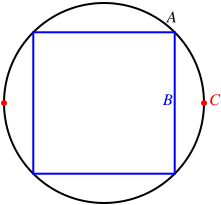
\includegraphics{HM_Example}}
\caption{Sets $A$, $B$, and $C$.}
\label{F:Hausdorff_Example}
\end{center}
\end{figure}
	\ba
	\item Find $h(A,B)$. 
	
	

\begin{comment}

In this case, $d(A,B) = d_E\left((0,1),\left(0, \frac{1}{\sqrt{2}}\right) = \frac{1}{\sqrt{2}} = d(B,A)$. So $h(A,B) = \frac{1}{\sqrt{2}}$.

\end{comment}
 	
	\item Find $h(A,C)$.
	
	

\begin{comment}

In this case, $d(C,A) = 0$ since $C \subset A$. However, $d(A,C) = d_E\left((0,1),(1,0) = \sqrt{2}$. So $h(A,C) = \sqrt{2}$. 

\end{comment}
	
	\item Find $h(B,C)$. 
	
	

\begin{comment}

In this case, $d(C,B) = d_E\left((1,0), \left(\frac{1}{\sqrt{2}}, 0\right) \right) = 1-\frac[1}{\sqrt{2}}$ while $d(B,C) = d_E\left(\left(0, \frac{1}{\sqrt{2}}\right), (1,0)\right) = \sqrt{3}{2}$. So $h(B,C) = \sqrt{3}{2}$. 

\end{comment}
	
	\ea
\end{activity}



Activity \ref{act:Hausdorff_example} indicates that the fact that $A$ and $B$ are compact sets allows us to find specific elements $a \in A$ and $b \in B$ so that $d_E(a,b) = d(A,B)$ and thus achieve maximum and minimum values in our definition of the Hausdorff metric. The proof that $h$ is a metric is well-known (see \cite{Barnsley, Edgar} for example). 

\begin{comment}
The only property that requires significant work is the triangle inequality. 

To prove the triangle inequality, let $A,B,C$ be compact subsets of a metric space $(X,d)$. We know that either $h(A,C) = d(A,C)$ or $h(A,C) = d(C,A)$. Without loss of generality, assume $h(A,C) = d(A,C)$. Choose $a \in A$ such that $d(a,C) = d(A,C) = h(A,C)$. Now choose $c \in C$ such that $d_E(a,c) = d(a,C) = h(A,C)$.  

Let $b_a \in B$ and $c_a \in C$ such that $d_E(a,b_a) = d(a,B)$ and $d_E(b_a, c_a) = d(b_a,C)$. Since $d_E(a,c) = \min_{c' \in C} \{d_E(a,c')\}$, we know $d_E(a,c) \leq d_E(a,c_a)$. The triangle inequality for the Euclidean metric gives us 
\[h(A,C) = d(A,C) = d_E(a,c) \leq d_E(a,c_a) \leq d_E(a,b_a) + d_E(b_a,c_a) = d(a,B) + d(b_a,C).\]
Since $d(a,B) \leq d(A,B)$ and $d(b_a,C) \leq d(B,C)$, we have 
\[h(A,C) \leq d(A,B) + d(B,C) \leq h(A,B) + h(A,C).\] 
\end{comment}


\csection{The Digital Line Topology}

``The main purpose of Digital topology is the study of topological properties of discrete
objects which are obtained digitizing continuous objects. Digital topology plays a very
important role in computer vision, image processing and computer graphics. The ultimate
aim of this article is to analyze the behavior of various general topological concepts in the
Khalimsky topology. In this article, we provide some results and examples of topology on
Z, the set of all integers. Also, we explain the concepts of digital line and digital intervals
with illustrative counterexamples."

Digital topologies. Main idea is to mimic the continuous information from the digital data. We restrict our discussion to two dimensional space. A continuous image can be represented in $\R^2$, as the curve in Figure \ref{F:DT_cont}. However, if we only have digital information in a data set, say information that is sampled from the continuous image as in the points shown on the graph in Figure \ref{F:DT_cont}, then we work in a discrete space. Each point in our data set is called a \emph{pixel} and to each pixel we assign a point with integer coordinates. In this way our discrete space is represented as $\Z^2$. 

In the continuous case, any open ball $B(x,r)$ with positive radius in $\R^2$ contains 

Let  $\tau$ be the topology on $\Z$ with basis $\{B(n)\}$, where 
\[B(n) = \begin{cases} \{n\}	&\text{if $n$ is odd}, \\ \{n-1,n,n+1\}	&\text{if $n$ is even}. \end{cases}\]
This topology is called the \emph{digital line topology} and has applications in digital processing.\footnote{See \emph{Introduction to Topology: Pure and Applied} by Colin Adams and Robert Franzosa , Pearson Education, Inc., 2008,  Sections 1.4 and 11.3.} The set $\Z$ with the digital line topology is called the \emph{digital line}. 

%Remove from activity in Closed sets topology section

